\chapter{Introduction}

Calcium in the form of $Ca^{2+}$ ions is a life and death signal, acting as an intracellular messenger in the body, carrying information in cells to regulate their activity \shortcite{Berridge}. {$Ca^{2+}$ signals are relevant to many cell functions, for example muscle contractions and cell adhesion \shortcite{Berridge}. } In this project, we study mathematical modelling of $Ca^{2+}$ signalling in fertilisation of the mammalian egg. Our focus will be on deterministic, spatially homogeneous models, paying close attention to the dynamics of the $IP_3$ receptors ($IP_3R$). After studying the existing models and experimental data available, we derive a new model that successfully captures many of the key features that regulate $Ca^{2+}$ signalling in a fertilising egg. 

\section{$Ca^{2+}$ signalling in fertilisation}

The cytosolic $Ca^{2+}$ concentration in almost every cell type is carefully controlled by sophisticated mechanisms \shortcite{Berridge2000}. As a result, the $Ca^{2+}$ shows complex spatiotemporal behaviour \shortcite{atri,swann2013,wallingford2001}. These behaviours range from stochastic spiking, to regular oscillations, periodic waves, and spiral waves. {The ECF has a $Ca^{2+}$ concentration of around $1 mM$, while active pumps and exchangers maintain the concentration of cytoplasmic $Ca^{2+}$ at around 0.1 μM.} Some intracellular compartments, for example the endoplasmic reticulum (ER) and mitochondria, have a comparatively high concentration of $100-800\mu M$ \shortcite{cellcalcium}. High levels of cytosolic $Ca^{2+}$ for prolonged periods of time can be cytotoxic \cite{Berridge2000}, hence $Ca^{2+}$ regulation is very important. In this project, we aim to model $Ca^{2+}$ signalling in fertilising eggs. During fertilisation, $Ca^{2+}$ oscillations are {triggered} by $PLC_{\zeta}$ and are the essential trigger of embryo development. $PLC_{\zeta}$ is a testes-specific isoform of phospholipase C ($PLC$) and is located in the sperm cytoplasm. $PLC$ is an enzyme that is restricted to the plasma membrane}.  The number of $Ca^{2+}$ oscillations influences the rate of embryo development \cite{swannlai}. These $Ca^{2+}$ oscillations have a large amplitude ($1 \mu M$) and low frequency (time period $>$10 mins). The initial $Ca^{2+}$ increase lasts approximately five minutes. Each subsequent $Ca^{2+}$ rise is very rapid (1 sec) and the $Ca^{2+}$ increases last for about 1 minute. $Ca^{2+}$ oscillations in a fertilising mouse egg can be seen in {Figure \ref{karlfig2}.

\begin{figure}[h!!!t!!!b!!!p]
  \centering
  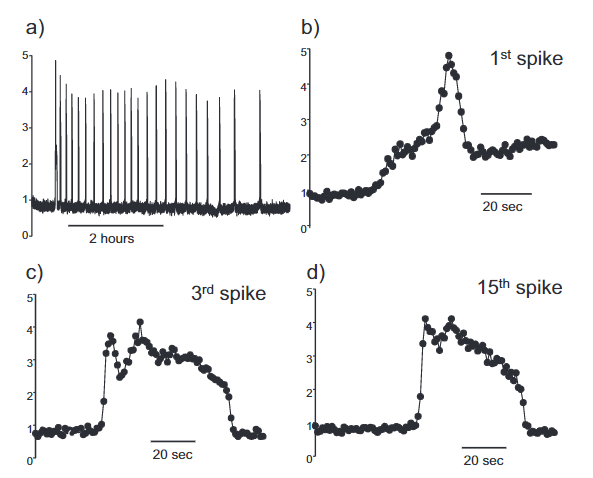
\includegraphics[width=\linewidth]{Chapters/1_Introduction/extras/karlfig1.png}
  \caption{Intracellular $Ca^{2+}$ oscillations in a fertilising mouse egg. This is measured by the fluorescence of the $Ca^{2+}$-sensitive dye Rhod dextran. The fluorescence is plotted as a ratio of the fluorescence
versus time divided by the starting fluorescence. Once the sperm is added there are large increases in fluorescence ratio
indicating $Ca^{2+}$ increases in the cytoplasm. The amplitude of the $Ca^{2+}$ oscillations is variable and likely to be in the range of $1-2 \mu M$ \shortcite{swann2013}. {Source:} \citeA{swann2013}. }\label{karlfig2}
\end{figure}

\subsection{Agonists, receptors and second messengers}

The most important of the signalling pathways is the phosphatidylinositol signalling pathway \cite{Berridge2000}. Here, {in a somatic cell,} phospholipase C ($PLC$) is activated and splits another membrane molecule, phosphatidylinositol 4,5-bisphosphate ($PIP_2$), into inositol 1,4,5-triphosphate ($IP_3$) and diacylglycerol (DAG). The $IP_3$ that is released into the cytosoplasm  then binds to $IP_3$ receptors ($IP_3R$) which lie on the membrane of the endoplasmic/sarcoplasmic reticulum (ER/SR). The $IP_3R$ are channels that release $Ca^{2+}$ from the $ER$ to the cytosol \shortcite{parys1995}.

In fertilisation, once sperm has fused with the egg membrane, the sperm $PLC_{\zeta}$ {(an isoform of $PLC$)} diffuses into the egg cytoplasm. Here, the $PLC_{\zeta}$ binds to $PIP_2$ which leads to the generation of $IP_3$. This $IP_3$ binds to the $IP_3R$ on the ER, causing the ER to release $Ca^{2+}$. The increase in $[Ca^{2+}]$ in the cytosol then stimulates the activity of $PLC_{\zeta}$ to generate more $IP_3$. Therefore, as $PLC_{\zeta}$ diffuses across the egg, this positive feedback loop occurs throughout the cytoplasm \cite{swannlai}.

\begin{figure}[h!!!t!!!b!!!p]
  \centering
  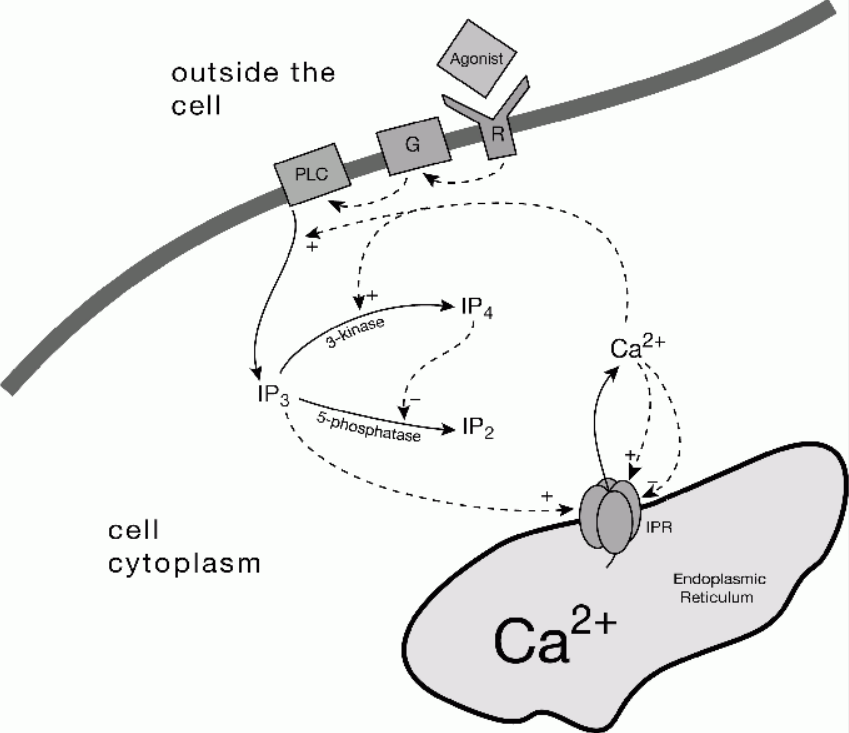
\includegraphics[width=0.7\linewidth]{Chapters/1_Introduction/extras/toolbox.png}
  \caption{A schematic of the PLC pathway for $Ca^{2+}$ signalling. R - Receptor, G - GPCR. Source: \citeA{sneyd2007}.}\label{sneydcatoolbox}
\end{figure}

\begin{figure}[h!!!t!!!b!!!p]
  \centering
  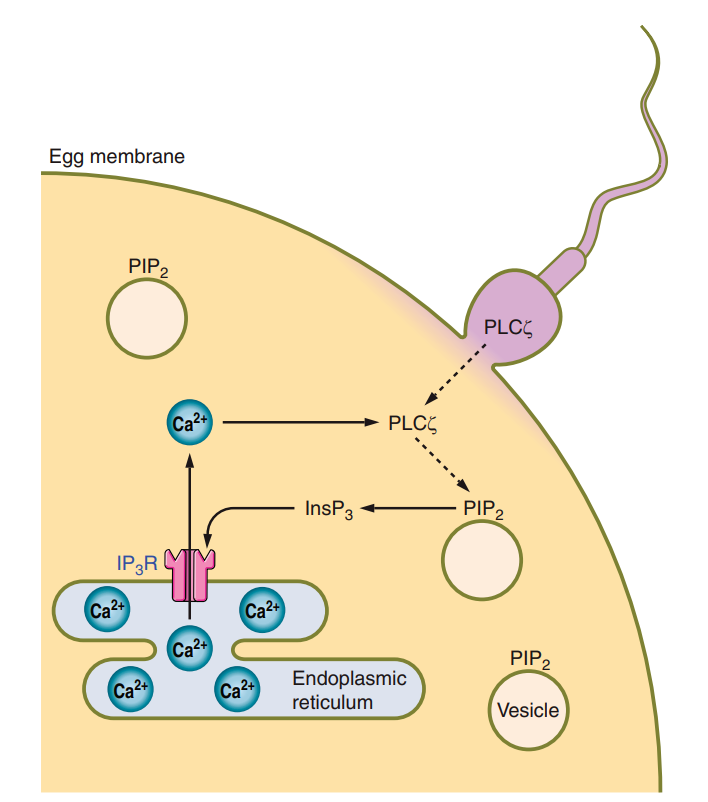
\includegraphics[width=0.6\linewidth]{Chapters/1_Introduction/extras/karlfig6.png}
  \caption{A schematic diagram showing the proposed mechanism of action of $PLC_{\zeta}$ during fertilisation. Once sperm has fused with the egg membrane, the sperm $PLC_{\zeta}$ diffuses into the cytoplasm. It then binds to $PIP_2$ and this leads to the generation of $IP_3$. $IP_3$ binds to the $IP_3R$ on the ER and this causes $Ca^{2+}$ release from the ER. Source: \citeA{swannlai}. }\label{sneydcatoolbox}
\end{figure}

\subsection{Internal compartments}
The most significant of intracellular compartments when it comes to $Ca^{2+}$ signalling is the ER \shortcite{berridgegalione1988}. Its main function concerns protein synthesis, and it makes up approximately $10\%$ of the total cellular volume. The ER is able to store a substantial amount of $Ca^{2+}$, and release it into the cytosol very quickly. The large amount of $Ca^{2+}$ enters the ER via the sarcoplasmic/endoplasmic reticulum $Ca^{2+}$ ATPases (SERCA) pumps, and escapes through two major types of receptor $Ca^{2+}$ channels \shortcite{marks1997}. These are the $IP_3R$ and the ryandine receptor (RyR).

The mitochondria in the cell are responsible for producing adenosine triphosphate (ATP) and also act as a $Ca^{2+}$ store. It is still not well understood how the mitochondria interact with cytosolic $Ca^{2+}$. It is highly suspected that the ER is the main driving force for the intracellular $Ca^{2+}$ fluxes, while the mitochondria might play a more passive modulatory role \shortcite{Jouavilleetal1995}.

\subsection{Internal calcium channels}

As described above, $Ca^{2+}$ is released from the ER through two types of receptors. The RyR is the largest known ion channel \shortcite{VanPetegem2012, FillandCopello2000}. It is mainly found in cells other than eggs, such as cardiac cells and skeletal muscle cells. For this reason we do not go into further depth regarding this channel.

The second major intracellular $Ca^{2+}$ channel is the $IP_3$ receptor ($IP_3R$) \shortcite{josephs, Pateletal1999, TaylorandLaude2002, Foskett2007, Mak2015}. The probability of the $IP_3R$ being open is referred to throughout this thesis as the \textit{`open probability'} ($P_O$). At low cytosolic $Ca^{2+}$ levels, an increase in the $Ca^{2+}$ concentration leads to an increase in $P_O$. This starts a positive feedback process of $Ca^{2+}$, known as $Ca^{2+}$-induced $Ca^{2+}$ release (CICR). At higher levels of $Ca^{2+}$ concentration, $P_O$ begins to decrease. In other words, the steady-state value of $P_O$ is a biphasic function of $Ca^{2+}$ \shortcite{parysetal}. Figure \ref{biphasicsketch} shows a graph of this based on experimental data \shortcite{Mak1998}. The $IP_3R$ is also affected by $IP_3$. An increase in cytosolic $IP_3$ concentration also increases $P_O$. We will go into further detail about this later as the $IP_3R$ mechanisms and dynamics are a main feature of this thesis.

\begin{figure}[h!!!t!!!b!!!p]
  \centering
  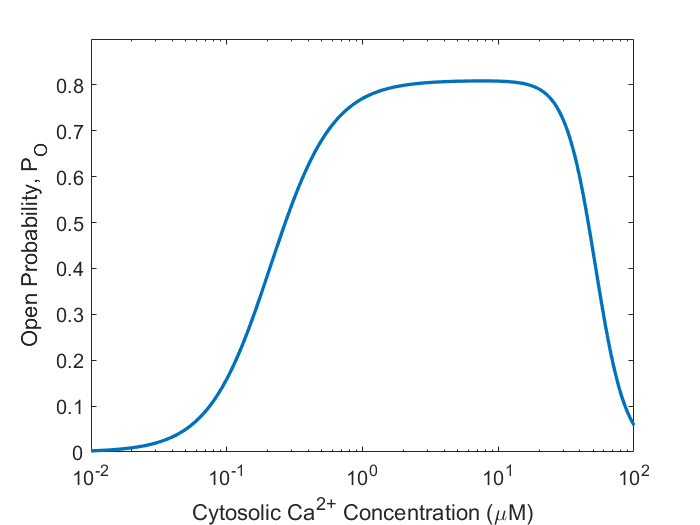
\includegraphics[width=0.65\linewidth]{Chapters/1_Introduction/extras/biphasicsketch.png}
  \caption{The open probability of the $IP_3R$, $P_O$, as a function of the cytosolic $Ca^{2+}$ concentration ($\mu M$). This was plotted at an $IP_3$ concentration of $0.1 \mu M$ using the equation for $P_O$ and data from \citeA{Mak1998}. \textit{Software}: MATLAB. }\label{biphasicsketch}
\end{figure}

We have touched on the basics of $Ca^{2+}$ signalling, and the schematic in Figure \ref{sneydcatoolbox} provides a visual description of those. However, other aspects are specific to the type of cell considered.

Many studies and experiments have been carried out on the fertilisation of an aquatic frog (Xenopus Laevis), for example \shortciteA{busa, nuccitelli, fontanilla}. The diameter of their oocytes can be larger than {$600\mu M$}, around $50-100$ times larger than an average cell (\shortcite{dupont}, page 23). Their greater size means they are perfect for experimental investigations of $Ca^{2+}$ signalling. {Immature Xenopus oocytes show complex spatiotemporal organisation \shortcite{Lechleiter1991}, forming concentric circles and multiple spirals. A typical $Ca^{2+}$ wave in a smaller cell cannot be observed in its entirety. Furthermore, there is not enough room for a spiral to form, and so $Ca^{2+}$ waves take a form that is almost planar. In a larger cell like the Xenopus oocyte, it is possible to observe both the wave front and wave back, as well as spiral waves.} $Ca^{2+}$ blips and puffs are evoked by very low levels of $IP_3$, while oscillations are observed in immature oocytes in response to sufficient amount of caged $IP_3$ \shortcite{marchant1999}. These oscillations correspond to the repetitive $Ca^{2+}$ waves that propagate throughout the cell during fertilisation \shortcite{berridge1994, thomas1996}.

Upon fertilisation of an egg, sperm-egg fusion yields an alternative type of $Ca^{2+}$ response in the way of a single slow $Ca^{2+}$ wave inside the egg. It takes about four minutes for the wave to traverse the egg, with a high level of $Ca^{2+}$ concentration maintained for the next $5-6$ minutes after the propagation \cite{fontanilla}. It is fortunate that there are detailed experimental data on Xenopus oocytes and on the elements of the $Ca^{2+}$ toolbox that are relevant for eggs. The Xenopus egg is very similar to mammalian eggs, particularly in the type of $IP_3R$ present which is a type 1 $IP_3R$. We also have accurate data of the $IP_3R$ dynamics \cite{Mak1998}. These data provide us with the opportunity to develop a new model that captures key features of the $Ca^{2+}$ dynamics in the fertilisation of a mammalian egg. Such a model, to the best of our knowledge, does not exist in the literature.

\section{Mathematical models for $Ca^{2+}$ signalling}

Models of $Ca^{2+}$ signalling can be divided into four major subgroups.  Firstly, they can be divided into deterministic and stochastic models, and secondly they can be divided into spatially homogeneous (ordinary differential equations, or ODEs) and spatially distributed models (partial differential equations, or PDEs). $Ca^{2+}$ signalling is intrinsically stochastic and spatially distributed \shortcite{sun1998, callamaras2000, falke2003}. This makes the mathematical analysis of $Ca^{2+}$ signals quite difficult. However, deterministic models can be useful for making predictions while they are easier to solve numerically than analogous stochastic models and so they remain a highly useful tool. In many cases, these predictions can (and have been) supported by experimental evidence and have been used extensively \cite{atri,deyoungkeizer,dupont1998}. For example, in \shortciteA{shuai} the deterministic \shortciteA{lirinzel} model is compared to two stochastic models and found to agree well when the number of $IP_3R$ is large enough.

There is a spatial aspect to the $Ca^{2+}$ oscillations at fertilisation, but the purely $IP_3$ induced $Ca^{2+}$ oscillations, in oocytes, that we will model are uniform across the egg with no obvious wave. This was shown in imaging experiments \shortcite{carroll}. We will therefore focus on deterministic, spatially homogeneous models, as a first approach to our challenge of creating a new model for $Ca^{2+}$ signalling in fertilising eggs. 

Figure \ref{classicmodel} shows the $Ca^{2+}$ fluxes in a cell. These fluxes are the following: into the cytosol through $IP_3R$ from the $ER$ ($J_{channel}$), out of the cytosol into the ER ($J_{pump}$), into cytosol through leak from the $ER$ ($J_{leak}$), into the cell ($J_{in}$), and out of the cell ($J_{pm}$).  We can define an ODE which represents the change in $Ca^{2+}$ concentration in the cytosol over time, as follows:
\begin{align}
    \frac{dc}{dt}=J_{channel}-J_{pump}+J_{leak}+(J_{in}-J_{pm}),\label{c}
\end{align}
where $c$ represents the cytosolic $Ca^{2+}$ concentration ($\mu M$). {In the ODE above, each $J$ flux represents the impact on the concentration within the cell due to the flux into or out of the cell, rather than the true flux that we see in Figure \ref{classicmodel}. The units of flux in the ODE are {$\mu M s^{-1}$}. We later show how true fluxes are translated into changes in concentration due to those fluxes using equation \eqref{converted}. } Note that throughout this project, when referring to $Ca^{2+}$ concentration, we are referring to the concentration in the cytosol unless stated otherwise. Each type of flux can actually be modelled in different ways \cite{sneyd2007}, depending on which elements are relevant. 

In this thesis, we pay close attention to the so-called gating models. These are models which include one ODE for $[Ca^{2+}]$, as given in equation \eqref{c}, and an ODE that models the proportion of non inactivated (or `\textit{openable}') $IP_3R$, $n$. This means that some $IP_3R$ are fully inactivated (and cannot be opened), and the other $IP_3R$ are closed but not inactivated, so can be opened. We wish to avoid the cytosolic $Ca^{2+}$ oscillations depending on the ER $Ca^{2+}$ store depleting as experimental evidence suggests that this does not drive oscillations during fertilisation \shortcite{Sanders2018,wakai}. The equation for the proportion of non inactivated $IP_3R$, $n$, is given as follows:
\begin{align}
    \tau_n\frac{dn}{dt}=n_{\infty}(c)-n,\label{n}
\end{align}
where $n_{\infty}$ represents the steady state of $n$ as a function of $c$, and $\tau_n$ is a time scale.

\begin{figure}[h!!!t!!!b!!!p]
  \centering
  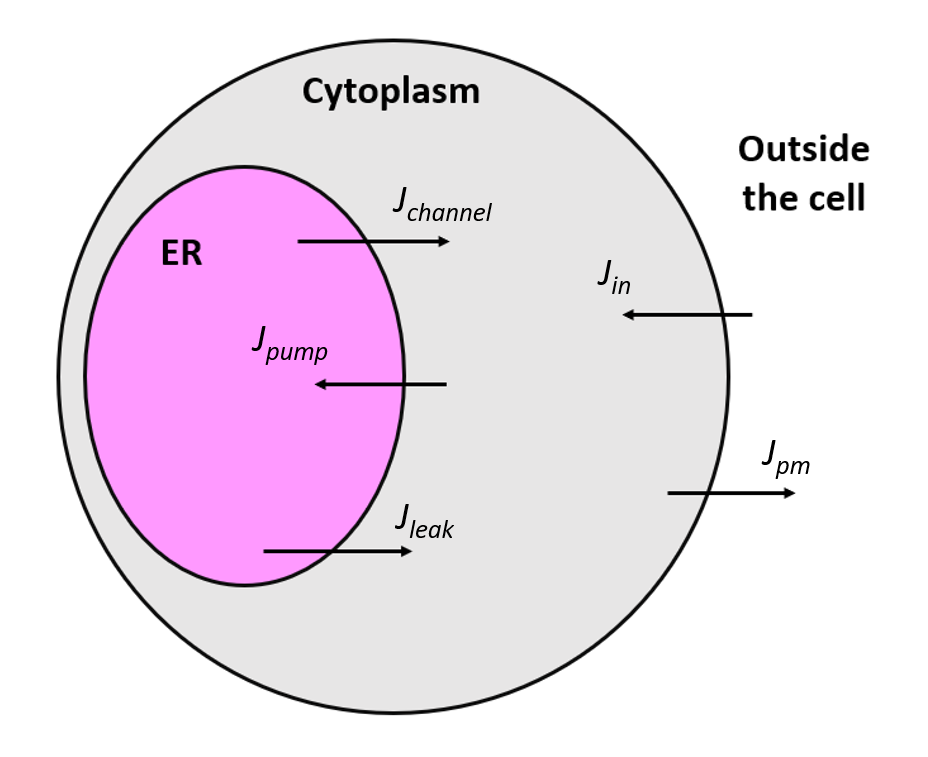
\includegraphics[width=1\linewidth]{Chapters/1_Introduction/extras/classicmodel.PNG}
  \caption{A diagram illustrating the fluxes in and out of the cell's cytoplasm typically modelled in a gating model, as in ODEs \eqref{c} and \eqref{n}. Flux into the cytosol through $IP_3R$ from the ER is represented by $J_{channel}$. Flux out of the cytosol back into the ER through SERCA pumps is represented by $J_{pump}$. There is also a leak of $Ca^{2+}$ from the ER into the cytosol represented by $J_{leak}$. Flux into and out of the cytoplasm over the cell plasma membrane is represented by $J_{in}$ and {$J_{pm}$}, respectively.}\label{classicmodel}
\end{figure}

Alternatively, equation \eqref{c} is commonly coupled with a second ODE to account for the change in $Ca^{2+}$ in the ER over time but this is not appropriate for modelling $Ca^{2+}$ signalling in fertilisation since oscillations should not be driven by the $Ca^{2+}$ store in the ER emptying \shortcite{Sanders2018,wakai}. This equation is presented as follows:
\begin{align}
    \frac{dc_e}{dt}=\gamma(-J_{channel}+J_{pump}-J_{leak}),\label{ce}
\end{align}
where $c_e$ represents $Ca^{2+}$ concentration in the $ER$. {$Ca^{2+}$ in the ER oscillates passively in the case of fertilisation, so parameter values can be tuned such that \eqref{ce} is approximately in steady state.} The parameter $\gamma$ represents the ratio of the volume of cytoplasm over the volume of the $ER$. This parameter is necessary since the volume of the ER is far less than that of the cytoplasm, making up just $10\%$ of the total volume of the cell. This means that the flow of $Ca^{2+}$ into the ER will cause a larger change in concentration in the ER than the flow of $Ca^{2+}$ into the cytoplasm.

Generally,  the ODEs \eqref{c}, \eqref{n} and/or \eqref{ce} can be coupled with other equations that could represent the state of the $IP_3R$, the states of the ATPase pumps, the $Ca^{2+}$ buffers, or the $IP_3$ concentration, amongst others \shortcite{atri, deyoungkeizer, dupontetal1991, hofer1999}.

We now briefly discuss the collection of models that have been constructed for $Ca^{2+}$ signalling. One type of model for $Ca^{2+}$ signalling is based on the assumption that the $Ca^{2+}$ concentration in the ER remains constant as the store is quickly refilled from the {cytoplasm} (\citeA{dupont}, page 104). {A model based on the ER refilling} was derived by \citeA{dupontgoldbeter1993}. Positive feedback of $Ca^{2+}$ release is assumed, and this drives the $Ca^{2+}$ oscillations. This type of model was developed before the dynamics of the $IP_3R$ were discovered and therefore does not account for any $Ca^{2+}$-dependent inactivation of the $IP_3R$. The model relies on depletion of the ER $Ca^{2+}$ store and the time period for oscillations is based on the time taken to refill the ER. One major problem that commonly occurs still in modern models is that the oscillations are assumed to emerge due to the ER store depleting and refilling. {Experimental data from \shortciteA{Sanders2018, wakai} suggests that this is not the case for eggs.}

{One of the early models} for the Xenopus oocyte was a gating model by \citeA{atri}. We will refer to this as the `Atri model' throughout this thesis. It is a simple, non-linear two--variable ODE model that gives rise to $Ca^{2+}$ oscillations. The model is highly cited and still regarded to be very relevant today. The model is studied in detail in Chapter 2. 

\citeA{deyoungkeizer} {derived a model} which we refer to as the `De Young-Keizer model'. Their kinetic model was based on experimental data on the $IP_3R$. It reproduces several in-vivo and in-vitro experimental results \shortcite{berridge1989,Mouillac1990,Smrcka}. It has nine variables and assumes a positive-feedback mechanism of $Ca^{2+}$ on $IP_3$ production.

Li and Rinzel developed a gating model by reducing the De Young-Keizer model, using the multiple scales method, to just two ODEs \cite{lirinzel}. We refer to this as the `Li-Rinzel model'. Like in the Atri model, the variables are the cytosolic $Ca^{2+}$ concentration and the proportion of non-inactivated $IP_3R$. This is another well-known gating model. The derived model retains the key features of the original De Young-Keizer model. We will take a thorough look at the Li-Rinzel model also in Chapter 2. 

In the Xenopus oocyte, the intracellular waves exhibit complex spatiotemporal organisation \shortcite{Lechleiter1991}. In order to take the first step towards modelling $Ca^{2+}$ waves in fertilising eggs, here we develop a deterministic gating (ODE) model for $Ca^{2+}$ oscillations which accurately reproduces key experimental features in fertilising eggs. {Previously, all models have incorporated $IP_3R$ dynamics that depend on $[Ca^{2+}]$ and $[IP_3]$ in an inaccurate manner, and some rely on the ER store depleting and refilling to drive oscillations. Evidence \shortcite{Sanders2018,wakai} suggests that this refilling is not the main driving force for oscillations in fertilisation and that they are mainly driven by the $IP_3R$ dynamics as published by \shortciteA{Mak1998}. We will derive a new model that incorporates the dynamics based on this more accurate data for how the $IP_3R$ dynamics depend on $[Ca^{2+}]$ and $IP_3$.}

\section{Project aims}

In this thesis we study a series of the well-known deterministic, spatially homogeneous $Ca^{2+}$ signalling models. We investigate how they work, paying close attention to the $IP_3R$ dynamics that are known to be the driving force for oscillations. There is currently, to our knowledge, no $Ca^{2+}$ model for fertilisation that contains the {accurate} type 1 $IP_3R$ dynamics {depending on $[Ca^{2+}]$ and $[IP_3]$} {according to the data} from \citeA{Mak1998}. Instead, many models for fertilisation rely on incorrect $IP_3R$ dynamics and the ER $Ca^{2+}$ store emptying to drive oscillations.

Our ultimate aim for this project is to develop a realistic model for $Ca^{2+}$ oscillations that occur during fertilisation in mammalian eggs. The model should use the most current understanding of the mechanism of action of the type 1 $IP_3R$ and of $PLC_{\zeta}$. It should also reproduce the low frequency, large amplitude oscillations characteristic of fertilising mammalian eggs (shown in Figure \ref{karlfig2}). The type 1 $IP_3R$ dynamics from \citeA{Mak1998}, {that accurately show how the open probability depends on $[Ca^{2+}]$ and $[IP_3]$}, must be incorporated. The model should not rely on the emptying of $Ca^{2+}$ stores {to drive the cytosolic $Ca^{2+}$ oscillations. }\cite{Sanders2018}. We aim to obtain such a model where the amplitude and frequency of $Ca^{2+}$ oscillations increase as $[IP_3]$ increases, as per the experimental data from \citeA{Sanders2018} and \citeA{sneyd}.

This will be achieved by first studying several existing $Ca^{2+}$ signalling models, out of the hundreds in the literature \cite{dupont}. A subset of these are related to fertilisation \shortcite{atri, Sanders2018, Theodoridou2013}. Many of these models appear to work well, but assume inaccurate $IP_3R$ dynamics \shortcite{hofer,Theodoridou2013,Sanders2018}, and rely solely on the concept of ER store refilling as the driving force of the $Ca^{2+}$ oscillations. We will take a step back from these recent models, many of which have three, or more, dynamic variables, and more parameters capturing other complex processes happening in the cell. We aim to develop a simple, two--variable model that incorporates experimental data for the open probability of the $IP_3R$ by \citeA{Mak1998}. The Atri model was the first model developed for the Xenopus oocyte, but it is still a good model to start from {as it captures the $Ca^{2+}$ induced $Ca^{2+}$ release mechanism operated by the ER, though depends on inaccurate data for how the $IP_3R$ depends on $Ca^{2+}$ and $IP_3$.} It is also a gating model with $Ca^{2+}$ oscillations not driven by the ER store depleting, but by the presence of an ODE for the proportion of non-inactivated $IP_3R$, as required.

The $IP_3R$ are channels that open and close to allow $Ca^{2+}$ to pass from the ER into the cytosol. The flux of $Ca^{2+}$ through the $IP_3R$ is controlled by the probability of a single channel being open. The mechanism for the open probability of the $IP_3R$ was identified by \citeA{Mak1998}. These data have not been however, acknowledged sufficiently in recent $Ca^{2+}$ modelling. They display some interesting features in regards to the dependence of the open probability on $Ca^{2+}$ and $IP_3$. We will deepen our understanding of these dynamics and explore how they can be incorporated into a $Ca^{2+}$ model. We have been collaborating with Professor Karl Swann (Cardiff University), and his involvement has been crucial in this project. With insights from the Swann lab, we aim to present a new model, that accurately captures the $Ca^{2+}$ oscillations, while using the correct dynamics from \citeA{Mak1998}. This will emulate the data from \citeA{Sanders2018} and \citeA{sneyd} that tell us how the frequency and amplitude of $Ca^{2+}$ oscillations behaves when $[IP_3]$ is increased. In this way, we aim to capture some of the complex features of $Ca^{2+}$ signalling in eggs and in particular $Ca^{2+}$ oscillations.

The experimental data from the Swann lab (see \citeA{Sanders2018}) show that having $IP_3$ concentration as a dynamic variable is essential in a future model. In this work we set out to complete the initial important step towards this by deriving a two--variable model for $Ca^{2+}$ signalling in fertilising eggs with the inclusion of the $IP_3R$ dynamics from \citeA{Mak1998} where $IP_3$ is a bifurcation parameter. This is the first step to reaching a three--variable model (with $IP_3$) that could inform future experiments and ultimately IVF clinical practice.

\section{Thesis overview}

We follow an incremental approach in this thesis. Firstly, we review current $Ca^{2+}$ models and identify strengths and areas of improvement. We then analyse the true $IP_3R$ dynamics in accordance with the data from \citeA{Mak1998}, and the equation that describes them. With this, we will then derive a system, based on an existing model, ensuring the addition of the accurate $IP_3R$ dynamics. 

In Chapter 2 we review and analyse several existing $Ca^{2+}$ models, paying particular attention to those of \citeA{atri} and \citeA{lirinzel}. In this literature review we take note of the key features of each model, including investigating the $IP_3R$ dynamics and its open probability. We also recognise the role of $IP_3$ as a bifurcation parameter. This is an essential feature that has to be included in any future $Ca^{2+}$ model. In Chapter 3 we take a close look at the correct dynamics of the $IP_3R$ as determined by \citeA{Mak1998}. We examine the data and the fairly complex `biphasic Hill function' used in \citeA{Mak1998} to describe these data. We acknowledge previous inaccuracies in the modelling of the $IP_3R$ and improve them. In Chapter 4 we take a brief look at one model that has incorporated these dynamics already \shortcite{swedish} and discuss the relevance to our project.

In Chapter 5 we derive a new model - based on the Atri model but with the correct open probability equation derived from the data in \citeA{Mak1998}. {Deriving this new model} requires careful and thorough analysis of both the Atri model and the equation for the open probability. We solve the two--variable model numerically and we also perform linear stability analysis. This model matches key features of data from \citeA{Sanders2018} and \citeA{sneyd} which show that the frequency and amplitude of $Ca^{2+}$ oscillations increase as $[IP_3]$ is increases. In Chapter 6 we summarize our results propose future research directions.
